%% starting from
%% bare_jrnl_compsoc.tex
%% V1.4b
%% 2015/08/26
%%
%% (requires IEEEtran.cls version 1.8b or later)
%%
%%*************************************************************************
%% Legal Notice:
%% This code is offered as-is without any warranty either expressed or
%% implied; without even the implied warranty of MERCHANTABILITY or
%% FITNESS FOR A PARTICULAR PURPOSE! 
%% User assumes all risk.
%% In no event shall the IEEE or any contributor to this code be liable for
%% any damages or losses, including, but not limited to, incidental,
%% consequential, or any other damages, resulting from the use or misuse
%% of any information contained here.
%%
%% All comments are the opinions of their respective authors and are not
%% necessarily endorsed by the IEEE.
%%
%% This work is distributed under the LaTeX Project Public License (LPPL)
%% ( http://www.latex-project.org/ ) version 1.3, and may be freely used,
%% distributed and modified. A copy of the LPPL, version 1.3, is included
%% in the base LaTeX documentation of all distributions of LaTeX released
%% 2003/12/01 or later.
%% Retain all contribution notices and credits.
%% ** Modified files should be clearly indicated as such, including  **
%% ** renaming them and changing author support contact information. **
%%*************************************************************************

\documentclass[10pt,journal,compsoc,letterpaper]{IEEEtran}
\usepackage{tcolorbox}
\usepackage{wrapfig}
\usepackage[utf8]{inputenc}

% *** CITATION PACKAGES ***
%
\ifCLASSOPTIONcompsoc
  % IEEE Computer Society needs nocompress option
  % requires cite.sty v4.0 or later (November 2003)
  \usepackage[nocompress]{cite}
\else
  % normal IEEE
  \usepackage{cite}
\fi
% cite.sty was written by Donald Arseneau
% V1.6 and later of IEEEtran pre-defines the format of the cite.sty package
% \cite{} output to follow that of the IEEE. Loading the cite package will
% result in citation numbers being automatically sorted and properly
% "compressed/ranged". e.g., [1], [9], [2], [7], [5], [6] without using
% cite.sty will become [1], [2], [5]--[7], [9] using cite.sty. cite.sty's
% \cite will automatically add leading space, if needed. Use cite.sty's
% noadjust option (cite.sty V3.8 and later) if you want to turn this off
% such as if a citation ever needs to be enclosed in parenthesis.
% cite.sty is already installed on most LaTeX systems. Be sure and use
% version 5.0 (2009-03-20) and later if using hyperref.sty.
% The latest version can be obtained at:
% http://www.ctan.org/pkg/cite
% The documentation is contained in the cite.sty file itself.
%
% Note that some packages require special options to format as the Computer
% Society requires. In particular, Computer Society  papers do not use
% compressed citation ranges as is done in typical IEEE papers
% (e.g., [1]-[4]). Instead, they list every citation separately in order
% (e.g., [1], [2], [3], [4]). To get the latter we need to load the cite
% package with the nocompress option which is supported by cite.sty v4.0
% and later. Note also the use of a CLASSOPTION conditional provided by
% IEEEtran.cls V1.7 and later.

% Macros for proof-reading
\usepackage[normalem]{ulem} % for \sout
\usepackage{xcolor}
\newcommand{\ra}{$\rightarrow$}
\newcommand{\ugh}[1]{\textcolor{red}{\uwave{#1}}} % please rephrase
\newcommand{\ins}[1]{\textcolor{blue}{\uline{#1}}} % please insert
\newcommand{\del}[1]{\textcolor{red}{\sout{#1}}} % please delete
\newcommand{\chg}[2]{\textcolor{red}{\sout{#1}}{\ra}\textcolor{blue}{\uline{#2}}} % please change

% Put edit comments in a really ugly standout display
\usepackage{ifthen}
\usepackage{amssymb}
\newboolean{showcomments}
\setboolean{showcomments}{true} % toggle to show or hide comments
\ifthenelse{\boolean{showcomments}}
  {\newcommand{\nb}[2]{
    \fcolorbox{gray}{yellow}{\bfseries\sffamily\scriptsize#1}
    {\sf\small$\blacktriangleright$\textit{#2}$\blacktriangleleft$}
   }
   \newcommand{\version}{\emph{\scriptsize$-$working$-$}}
  }
  {\newcommand{\nb}[2]{}
   \newcommand{\version}{}
  }


\newcommand\magnus[1]{\nb{Magnus}{#1}}
\newcommand\eric[1]{\nb{Eric}{#1}}
\newcommand\paolo[1]{\nb{Paolo}{#1}}
\newcommand\grant[1]{\nb{Grant}{#1}}
\newcommand\rogardt[1]{\nb{Rogardt}{#1}}
\newcommand\daniela[1]{\nb{Daniela}{#1}}



% *** Do not adjust lengths that control margins, column widths, etc. ***
% *** Do not use packages that alter fonts (such as pslatex).         ***
% There should be no need to do such things with IEEEtran.cls V1.6 and later.
% (Unless specifically asked to do so by the journal or conference you plan
% to submit to, of course. )


% correct bad hyphenation here
\hyphenation{op-tical net-works semi-conduc-tor}


\begin{document}
%
% paper title
% Titles are generally capitalized except for words such as a, an, and, as,
% at, but, by, for, in, nor, of, on, or, the, to and up, which are usually
% not capitalized unless they are the first or last word of the title.
% Linebreaks \\ can be used within to get better formatting as desired.
% Do not put math or special symbols in the title.
\title{Impediments and Enablers for Shared Modeling and Virtual Verification in Automotive Model-Driven Software Ecosystems}
% Exploring Ecosystem Aspects for Shared Modelling and Virtual Verification of Control Systems in Automotive Model-Driven System Engineering
%
%
% author names and IEEE memberships
% note positions of commas and nonbreaking spaces ( ~ ) LaTeX will not break
% a structure at a ~ so this keeps an author's name from being broken across
% two lines.
% use \thanks{} to gain access to the first footnote area
% a separate \thanks must be used for each paragraph as LaTeX2e's \thanks
% was not built to handle multiple paragraphs
%
%\IEEEcompsocitemizethanks is a special \thanks that produces the bulleted
% lists the Computer Society journals use for "first footnote" author
% affiliations. Use \IEEEcompsocthanksitem which works much like \item
% for each affiliation group.

\author{S. Magnus Ågren,~Eric Knauss, Paolo Giusto, Grant Soremekun, Rogardt Heldal, Daniela Damian% <-this % stops a space
\IEEEcompsocitemizethanks{
% note need leading \protect in front of \\ to get a newline within \thanks as
% \\ is fragile and will error, could use \hfil\break instead.
\IEEEcompsocthanksitem Magnus, Eric, and Rogardt are with Chalmers $\mid$ University of Gothenburg, Sweden
\IEEEcompsocthanksitem Paolo and Grant are with GM, USA
\IEEEcompsocthanksitem Daniela is with University of Victoria, Canada
}% <-this % stops an unwanted space
\thanks{Manuscript received 2017}}
% note the % following the last \IEEEmembership and also \thanks - 
% these prevent an unwanted space from occurring between the last author name
% and the end of the author line. i.e., if you had this:
% 
% \author{....lastname \thanks{...} \thanks{...} }
%                     ^------------^------------^----Do not want these spaces!
%
% a space would be appended to the last name and could cause every name on that
% line to be shifted left slightly. This is one of those "LaTeX things". For
% instance, "\textbf{A} \textbf{B}" will typeset as "A B" not "AB". To get
% "AB" then you have to do: "\textbf{A}\textbf{B}"
% \thanks is no different in this regard, so shield the last } of each \thanks
% that ends a line with a % and do not let a space in before the next \thanks.
% Spaces after \IEEEmembership other than the last one are OK (and needed) as
% you are supposed to have spaces between the names. For what it is worth,
% this is a minor point as most people would not even notice if the said evil
% space somehow managed to creep in.



% for Computer Society papers, we must declare the abstract and index terms
% PRIOR to the title within the \IEEEtitleabstractindextext IEEEtran
% command as these need to go into the title area created by \maketitle.
% As a general rule, do not put math, special symbols or citations
% in the abstract or keywords.
\IEEEtitleabstractindextext{%
\begin{abstract}
Virtual verification promises measurable gains in productivity of automotive systems development, especially if supported by the shared modeling of ECUs (electronic control unit) and their components across the automotive ecosystem and supply chain, and throughout the software development process, long before ECUs and components become available as silicon.
Yet, large scale adoption of virtual verification has proven difficult.
By describing benefits, critical impediments, and crucial enablers, we provide help for overcoming such difficulties.

%150 word limit
%
%Submission
%
%Managing Software Platforms and Ecosystems: Call for Papers
%
%Manuscripts must not exceed 3,000 words including figures and tables, which count for 250 words each. Submissions exceeding these limits might be rejected without refereeing.
%
\end{abstract}

% Note that keywords are not normally used for peerreview papers.
%\begin{IEEEkeywords}
%\end{IEEEkeywords}
}


% make the title area
\maketitle


% For peer review papers, you can put extra information on the cover
% page as needed:
% \ifCLASSOPTIONpeerreview
% \begin{center} \bfseries EDICS Category: 3-BBND \end{center}
% \fi
%
% For peerreview papers, this IEEEtran command inserts a page break and
% creates the second title. It will be ignored for other modes.
\IEEEpeerreviewmaketitle



\IEEEraisesectionheading{\section{Introduction}\label{sec:introduction}}
% Computer Society journal (but not conference!) papers do something unusual
% with the very first section heading (almost always called "Introduction").
% They place it ABOVE the main text! IEEEtran.cls does not automatically do
% this for you, but you can achieve this effect with the provided
% \IEEEraisesectionheading{} command. Note the need to keep any \label that
% is to refer to the section immediately after \section in the above as
% \IEEEraisesectionheading puts \section within a raised box.


% Own commands
\newcounter{sidebar}
\newcommand{\sidebar}[1]{\refstepcounter{sidebar}Sidebar \thesidebar{}:\label{#1}}
\newcommand{\fig}[1]{\refstepcounter{figure}Figure \thefigure{}:\label{#1}}

% Figures
\begin{tcolorbox}[float*,title=\sidebar{bar:ecosys} Ecosystem Background,width=\textwidth, lower separated=false]
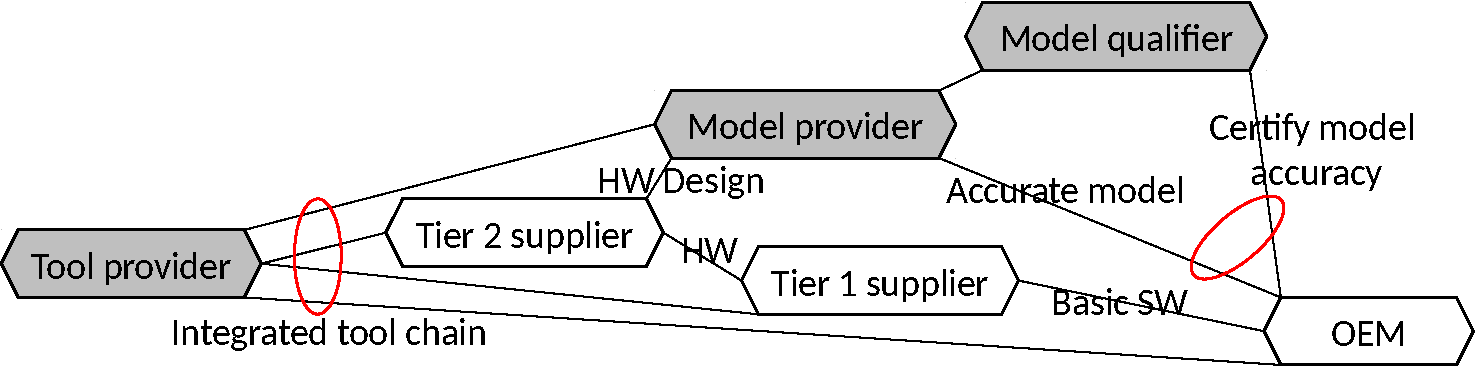
\includegraphics[width=\textwidth]{figures/ecosys}
\tcblower
The virtual platform technology ecosystem involves the model/tool suppliers, software/hardware IP suppliers, users, etc., and is described in \cite{Knauss2014d}.
The ecosystem is complex and may also involve the creation of new roles and responsibilities,
e.g., the standardization of the microprocessor model certification process  for accuracy and performance.
Ecosystem roles and responsibilities are similar in nature to those found in the ECU hardware ecosystem because there are mixed hardware and software IPs.
For hardware IP, the microprocessor core is often provided by a Tier-3 supplier who, in turn, provides this component to a Tier-2 micoprocessor provider
The same scenario applies to software IPs, with platform software modules provided by one vendor, device drivers provided by another vendor, and the microcontroller abstraction layer provided by the chip provider.
On top of these software layers, an OEM performs the overall integration.
%As expected the ecosystem here is quite complex.

A potential ecosystem for virtual platforms is shown \ins{above}.
The degree of granularity and the integration levels of the different IPs determines its complexity (e.g., integration of peripheral models into a microprocessor model, integration of microprocessor models and ASICs into an ECU model).
%As described earlier, other models/tools in addition to the virtual chipset simulator need to be integrated to accurately simulate the full functionality of the controller and configure the software image for testing via tools such as INCA.

Notation paper \cite{Sjaak Brinkkemper}
\end{tcolorbox}


\begin{tcolorbox}[float,title=\fig{fig:map} Map of Impediments and Enablers]
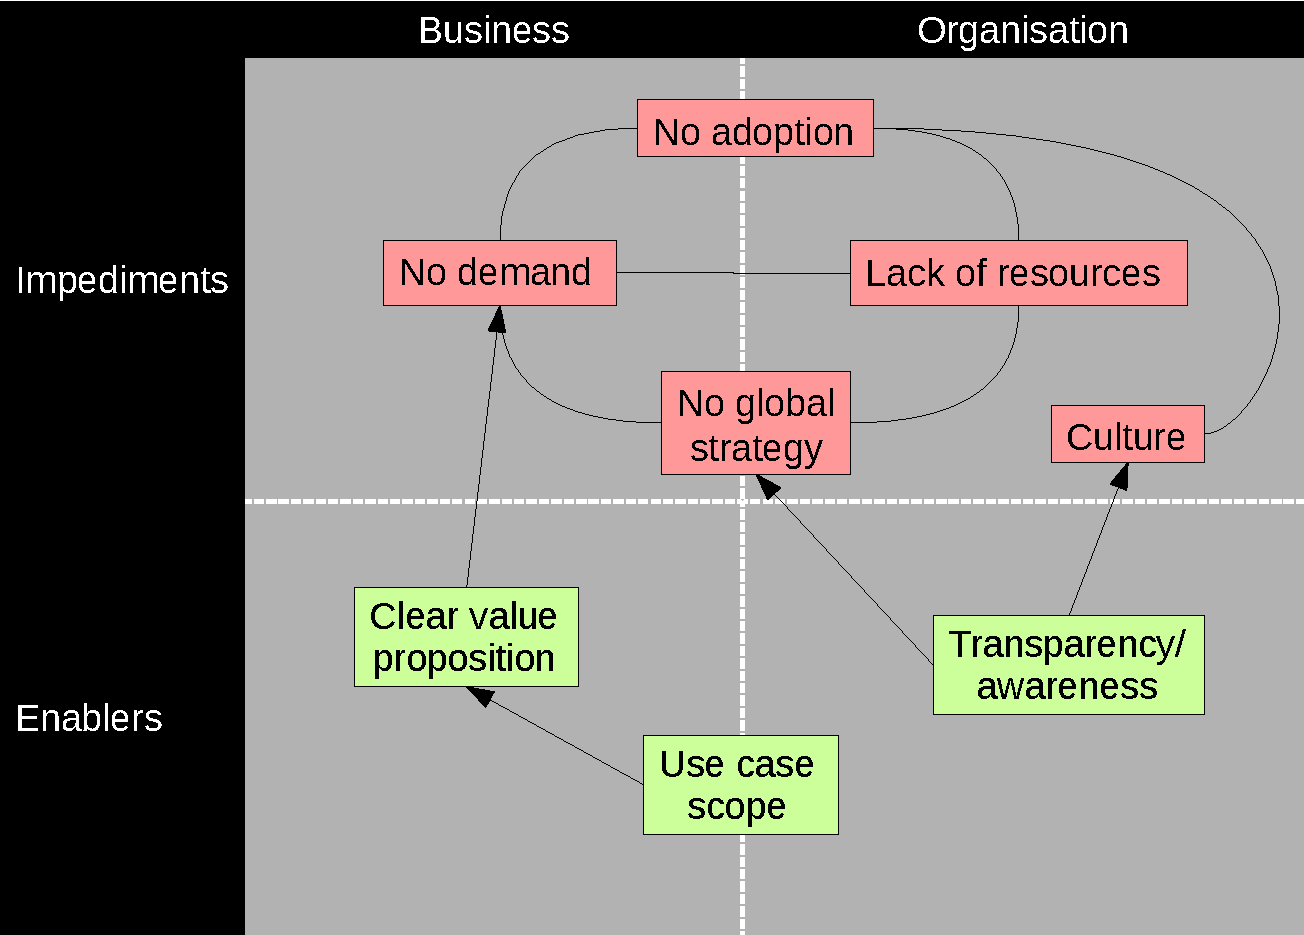
\includegraphics[width=\linewidth]{figures/results_map_simplified}
\end{tcolorbox}

\begin{tcolorbox}[float*,title=\sidebar{bar:tech} Technology Background,width=\textwidth]
  \begin{wrapfigure}{r}{0.6\linewidth}
  \begin{tcolorbox}[frame empty]
  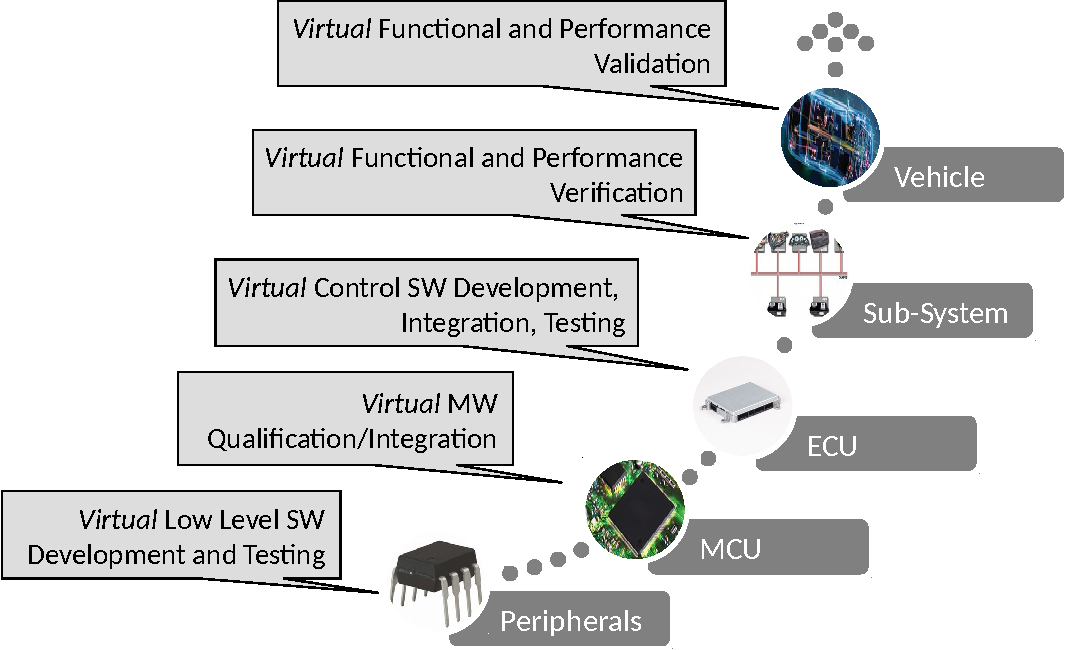
\includegraphics[width=\linewidth]{figures/virtual_platform}
  \end{tcolorbox}
  \end{wrapfigure}
The Virtual platform technology consists of two parts, a virtual chipset and a virtual platform for SW development, integration, and testing.
The Virtual chipset consists of a high-fidelity microprocessor model, including peripherals and other resources that execute the target embedded SW ("Target Code in the Loop").
Extending the virtual chipset with additional models of off chip devices essentially realizes the concept of a virtual controller.
Other models, similar to those required for hardware-in-the-loop/bench systems, are also required in order for the virtual controller to be able to emulate the behavior of the real controller's functionality and performance within a HIL bench.
These include models representing incoming serial data traffic, typically in open loop,
plant models (e.g., an engine), simulating ASICs running microcode, interfacing high power interfaces such as inductors to the controlled loads (e.g., electric motors, fuel injectors), HW/SW Fault Injection, vehicle dynamics, environment, etc.
The degree of modeling around the virtual chipset depends upon the use case at hand.
In order to perform a full functional and performance verification of the controller, all the aforementioned models are needed.
For use cases involving only low level SW development, an open loop model providing HW IOs and/or serial data traffic may be sufficient.
Finally, tools for configuring SW via calibrations and for SW variable/signal recording may also be needed. The integration of several virtual chip sets may be necessary for sub-system and/or complex ECU SW verification, and may require high-performance computing platforms to achieve acceptable simulation runtimes.

\end{tcolorbox}


% The development of automotive control architectures is increasingly dependent upon the use of modeling and simulation technologies.
% Use cases include the development of control algorithms and their related software implementations,
% of “platform” hardware/software architectures
% %(e.g., OEM ECU HW design \& integration, SW IP qualification and integration, LLHWIO SW development, etc.),
% and calibrations at the vehicle, subsystem, and hardware/software component level.
% Unfortunately, the general nature and history of automotive OEMs as large systems integrators of pre-allocated functionality to ECU hardware,
% often results in modeling and simulation technologies being deployed %(reactively)
% late in the development process
% %(e.g., at the HW/SW/Plant integration stage)
% and customized to specific use cases, domains, and/or organizations.
% There is a lack of standardized processes for tool/model integration and management across the OEM's engineering organizations. 
% The primary consequence of these problems is the OEM's struggle to design systems of ever-increasing complexity due to the growing number of errors,
% that often originate early in the conceptual and preliminary design phases, but aren't discovered until later during the hardware/software integration phase.
% Furthermore, the development speed of hardware and software components
% %(e.g., microcontrollers and software components)
% are limited by the supplier's own hardware and software development cycles.
% Thus, the integration of software and hardware can only be tested very late in the development cycle,
% further contributing to the possibility of costly software bugs and design errors.
% This leads to increased production delays and costly vehicle recalls, that significantly reduce product quality and profit margins.
% Finally, using component models and corresponding analysis and simulation tools to support the early verification and integration of control systems has not yet been widely accepted by OEMs
% -- or the automotive design community in general --
% as part of a standard development process.
% Currently, standard development processes are driven primarily by the exchange of tangible assets (ECUs, microcontrollers) and software IPs
% %(e.g., low lever device drivers),
% and not models of it, therefore preventing any opportunity of early integration.

%Understanding the underlying ecosystem of cross-organizational collaborations will allow us to properly articulate the challenges and benefits of designing electrical control architectures using shared modelling and virtual verification methodologies.

%\subsection{Availability of models vs. availability of hardware}
Virtual verification based on shared models is a strategy to manage the cone of uncertainty \cite{Boehm1981}, 
which says that uncertainty is gradually reduced as development progresses,
more information about the system becomes available,
and system integration aspects can be tested.
Many decisions need to be made in the beginning of the development process, though, when uncertainty is greatest.
Thus, the ability to give early feedback about design decisions is an important asset.
Consequently, any model characterizing hardware performance before the actual silicon hardware exists can be valuable in helping to develop the embedded software earlier.
%Once the hardware exists, models need to depict the hardware as closely as possible.
%A lack of accuracy is then hard to compensate by additional value of models over the real hardware, such as easy, location independent availability and scalability.

Several R\&D and engineering teams,
at a large North American OEM,
have been addressing the organizational and technical challenges related to the mainstream adoption of modeling and simulation technologies, for the virtual development and integration of electrical control architectures, to reduce the risk of late design changes.
The main area of progress has been the adoption of hardware-in-the-loop (HIL) benches,
coupling real time models of plants and of the rest-of-the-vehicle serial data traffic with real loads, sensors, and controllers.
Other areas of progress include software-in-the-loop (SIL) technologies, used to simulate the control behavior coupled with simpler real time models of plants.
Finally, high fidelity models of microprocessors running the real target controller code have been investigated.
While HIL benches are a mature area at the OEM, other areas exhibit technical and organizational challenges of various nature.
%In this article, we discuss some of the benefits, challenges, and enablers of modeling and simulation technologies for electrical control architecture,
%by analyzing the high fidelity modeling and simulation of processor technologies.
%We then generalize our findings to the more general area of modeling and simulation technologies for virtual development and integration.
%We believe that the work described in this article is of significance to any one
%at the OEM
%who is facing challenges, trying to "cross the chasm" from early niche adoption to main stream.
%By analyzing benefits, enablers, and impediments to adoption by means of interviews and workshops with relevant stakeholders in the ecosystem, we are able to identify potential ways to overcome the resistance to change, or at least possible ways to sell the value proposition.

%Model-based systems engineering aims to capture this information within a model that is managed throughout the product lifecycle. It is promising to extend these system models with relevant models on lower abstraction levels such as Microprocessor models that describe how ECUs are implemented. If connected, they would provide a bottom-up model for systems engineering, covering the automotive value chain (i.e. the process and activities that add value to an automotive system across OEM and suppliers), and allowing to reason about system aspects in a holistic way.

%Our findings indicate that virtual verification is a promising approach that could raise the overall maturity of developing software in the automotive ecosystem across organizational boundaries. We find that a systematic, model-based approach could enforce good system engineering practices throughout the ecosystem, and offer a holistic view on value creating engineering activities. If further confirmed, these results could support establishing an integrated model-based engineering approach at the whole vehicle level. While our research focusses on accelerating software development - we see this as one important sub-use cases and a step towards supporting a complete model-based approach that would allow to capture all relevant information in a (federated) system engineering model (e.g. SysML) and link it to engineering analysis and implementation downstream tools.


%we provide an overview of the technology area of focus.
The research presented in this paper is based on semi-structured interviews
with OEMs, suppliers, and tool vendors,
representing a cross-section of the automotive ecosystem,
and a follow-up workshop, with OEM personnel.

focused on the benefits and challenges of 
enterprise-scale deployment of MCU/ECU
%mixed fidelity
simulation models.

%Tie into impediments and enablers

\section{Benefits} \label{sec:benefits}
The potential benefits of shared modeling and virtual verification fall in two categories:
testing efficiency and collaborative advantages \emph{throughout the ecosystem}.

\subsection{Testing Efficiency}
\subsubsection{Earlier Software Integration Testing}
The main goal of virtual verification is to provide a means for testing the integration of software before the specific ECU/MCU hardware exists or before it is made available to the OEM.
%"Much earlier with virtual HW [...] Benefit for the OEM as testing could be done 1 year ahead"
%— Business Manager (Tier-2)
Earlier testing could also prove very valuable by identifying issues with the microcontroller specification if it is still evolving.
\begin{quote}
"[...] the specification of the MCU might be changing and therefore the model is still useful to find issues in the target embedded software as well as with the specification of the MCU. Economically, the initial investment should not be too large as the models are not required to be highly accurate because there still might be many bugs in the MCU specification. As long as SW development is progressing than there is significant benefit even if the model is not initially high fidelity."
-- CEO (Tool Vendor 1)
\end{quote}

\subsubsection{Easier Testing}
%Sharing microcontroller models for virtual verification may potentially have very positive effects on testing.
A virtual testing environment is generally easier to setup than a corresponding hardware based testing environment,
%(e.g., hardware in the loop (HIL) systems),
leading potentially to significant cost savings.
Hardware test benches are typically a heavily shared resource, resulting in scheduling conflicts and other logistic difficulties.
If models with sufficient fidelity were available, it would reduce the need to build and physically access hardware-based test benches, potentially reducing scheduling problems.
%Using ECU and MCU models also increases the visibility and controllability of the testing process.
%de-quoted
% Testing in the virtual environment is easier than the hardware environment because of the increased visibility of the microprocessor’s resources (e.g., Timing Processing Unit)
%— Business Manager (Tier-2)
Virtual boards also support parallelization, allowing for many tests to be executed in parallel assuming the host computers have enough processing power.
This could provide additional cost and time savings when compared to running tests on a physical board.
%"A simulator although slower than real time can actually be used in a much quicker fashion than a real vehicle bench to reproduce the problem."
%— CEO (Tool Vendor 1)

\subsubsection{Uncovering More Faults}
Virtual testing will allow engineers to monitor, control, and observe the testing environment in a more comprehensive manner than currently possible on physical hardware.
This includes easier ways to inject faults so that more thorough testing can be accomplished.
%These technologies could enable fault injection because they provide more visibility and controllability in the ECU HW resources. This could be done using the models while it can’t be done in general using the real HW.
%— Embedded Software/Tool Expert (Tier-1)
%Thus, a virtual testing environment could be a valuable asset that allows for the defining and maintaining of tools for fault injection and other advanced testing procedures.

\subsubsection{Hardware Dependent Regression Testing}
Virtual testing would simplify software regression tests on multiple (virtual) hardware platforms,
that do not need to be maintained across the entire product lifecycle.
%(assuming the models used for virtual testing have sufficient fidelity and reliability).
This could provide a cost-efficient way to ensure backward-compatibility for software patches,
or evolve software components in a product family.
%"Virtual benches could be useful except for target independent functional verification."
%— Software Development Leader 2 (OEM)
%Note: Software components must also be tested independently from the hardware platform, which is sufficiently addressed by existing software in the loop (SIL) and model in the loop (MIL) verification mechanisms.

\subsubsection{Repeatable Testing}
Relying on virtual regression testing would significantly improve repeatability.
%"[Virtual] Regression testing is much more powerful and repeatable using virtual testing platforms"
%— Business Manager (Tier- 2)
Having easily repeatable test procedures would allow for new and more efficient ways of developing (potentially target dependent) software.
Running regression tests more often in a defined environment could make it easier to find bugs earlier and reduce expensive recalls.
% \begin{quote}
% "In the traditional auto process typically it may take 6 months between when the SW bug is created and when the SW bug is detected! If you can switch from 6 months to 1 week cycle! This could be a breakthrough for the OEM."
% — Business Manager (Tier-2)
% \end{quote}

\subsection{Collaborative Advantages}
%In addition to increasing testing efficiency, shared modelling and virtual verification promises to support collaborations throughout the automotive ecosystem.

% \subsubsection{Within the OEM}
% The ability to do component level simulation and virtual verification across hundreds of developers promises to enable new ways of working and accelerate (continuous) software integration.
% %"Success stories include [...] component level simulations across 100+ users in [OEM]"
% %— Software Development Leader (OEM)
% Increasing design complexity makes it necessary for large numbers of engineers to have access to shared systems and engineering resources. A shared modeling and virtual verification capability will help address this necessity beyond what is typically in place today.

%\subsubsection{Within the Automotive Software Value Chain}
Shared modeling and virtual verification promises to improve and accelerate how suppliers develop software.
For example, if suppliers are encouraged to provide models and virtual assets early in the process to their customers (other suppliers and OEMs),
then they would likely embrace a model-first approach,
where models of their product are delivered first, integrated and verified upstream, before the development of hardware and low level software starts.
This would also benefit suppliers because it would encourage them to utilize model-driven development and virtual verification for their own internal processes.
%"One internal use case of shared modeling and virtual verification is HW verification at the RTL level in conjunction with emulation boxes."
%— Marketing Director (Tool Vendor 2)
By improving the awareness and the attractiveness of virtual verification technology across the complete ecosystem, the overall process and product quality can be improved, enabling Tier-1 and Tier-2 suppliers to fully benefit from model-driven engineering.

%\subsubsection{Across the Automotive Ecosystem}
In addition to facilitating collaboration between ecosystem actors, a shared modeling and virtual verification capability may also help facilitate the exchange of conceptual knowledge. This would provide feedback on system and software design and integration before hardware is available, significantly shortening the feedback cycle and enabling effective collaborative engineering much earlier in the design process.

% \begin{quote}
% "Tier-2 use cases are [either] internal or external and enable customers with three different use cases: (i) Internally, [the Tier-2 enables their] own internal MCAL SW development (ii) Also internally, [the Tier-2 enables] HW verification at the RTL level in conjunction with emulation boxes. Although these models are not meant to be used as SW development platforms, these models could be the starting point for it. (iii) Externally, [the Tier-2 enables collaboration] with their customers (typically Tier-1s)."
% -- Marketing Director (Tool Vendor 2)
% \end{quote}

%From the perspective of an OEM, these three use cases imply certain benefits:
Wide adoption of model-driven development practice among the Tier-2 suppliers could increase the modeling expertise throughout the automotive ecosystem.
The promise of re-using internally used models for verification, better integration, and alignment of model-driven development flows between
%Tier-1 and Tier-2
suppliers could decrease lead-time because:
(a) it mitigates the risk of potential delays in the delivery of actual ECU hardware and 
(b) it mitigates delays in developing the low-level software (which could progress even in the absence of the actual hardware).

% !TEX root = main.tex
\section{Impediments and Enablers}\label{sec:impediments_and_enablers}

Despite this great promise, bootstrapping a technological platform and critical relationships in an ecosystem for shared modeling and virtual verification has proven difficult thus far.
Our data shows, in line with more general theories on technology diffusion \cite{rogers2010diffusion} %\magnus{Covering diffusion/adoption in the sidebar mights save us a few words}
and technology transfer \cite{gorschek2006model}, that any effort to introduce shared modeling and virtual verification needs to take into account the larger context of the automotive domain and its value-chains. 
Our analysis of the data collected from the interviews sought to identify aspects of business, social (organizational), and technical nature, as suggested by Christensen et al. \cite{christensen2014analysis} and Tamburri et al. \cite{tamburri2013uncovering} for reasoning about ecosystems. 
%\eric{Here, I believe we need to make the ecosystem aspect visible. We are not looking at this problem as a technology diffusion problem. We are looking at it as a software ecosystem topic. Thus, we find a different way to approach the known difficulties.}. 
Figure \ref{fig:map} describes the impediments and enablers that we found in the business and organizational areas. 
While technical impediments were suggested to be of secondary importance by our data (and thus omitted from the figure), they do become %\chg{prominent}
{tangible} when deploying at scale.
%and \ugh{thus we describe them below}\eric{But they are now gone. I think we need them very shortly?}. \magnus{I suggest keeping them out, and dropping the forward reference.}

%\subsubsection{Technical Impediments}
%we recognize that complexity, variance, interoperability, scale, and similar impediments will be encountered and need to be addressed.
%\textbf{Potential technical impediments} include
%lack of \emph{model interoperability},
%challenges to \emph{keep models up-to-date} with evolving hardware,
%lack of \emph{trust in model fidelity},
%and lack of protection of \emph{intellectual property}.

%\subsubsection{Technical Enablers}
%Conversely, \textbf{foreseeable technical enablers} include a shared and standardized \emph{modeling platform},
%\emph{reusable model templates} for handling product line variation points,
%and increased standardization at the \emph{system architecture} level, for example of computational ECUs.



%\subsection{Business and Organization}
With respect to \textbf{business- and organization-related impediments}, Figure \ref{fig:map} shows an undesirable circular dependency:
since there is a \emph{lack of demand} for high-fidelity modeling technology,
there is also a \emph{lack of global strategy} for the use of virtual platform technology.
Without such a strategy, there is limited personnel available (\emph{lack of resources}),
which leads to \emph{lack of adoption}.
Consequently, there is no clear value proposition for widespread adoption of virtual platform technology, therefore making it difficult to generate enough demand.

% full circle before the below
The lack of adoption is further increased by a hardware-centric, conservative \emph{culture} that is accustomed to using HIL benches with physical controllers.

% enablers
As \textbf{business- and organization-related enablers}, %With respect to the enablers, 
we see a \emph{clear value proposition} as crucial to breaking the circular dependency and creating more demand.
This will be helped by clearly articulating customer value and by \emph{properly scoping use cases} based on a \emph{clear ecosystem landscape}.
These enablers also need to be mapped to an overall company strategy in order to facilitate wider adoption. 

A \emph{clear ecosystem landscape} and \emph{knowledge sharing} %\del{can mitigate} 
{is an essential enabler to address} the lack of global strategy.
The foundation of this is sharing knowledge about what capabilities are currently working, what benefits have already been achieved, and combining knowledge from different initiatives.
This will encourage grassroots adoption (e.g., from visionary engineers) and may in turn trigger wider adoption
%\chg{and then resources toward mainstream adoption. Transparency about benefits will also help to mitigate the cultural impediments.}
as well as increased availability of resources that would support mainstream adoption. Encouraging transparency about the potential benefits may also help mitigate cultural impediments.

\subsection{Impediments in Context}
We concretize the impediments 
\emph{lack of global strategy} and \emph{lack of resources}
by describing a specific scenario:
Modern automotive MCUs carry several core computing units, including specific time processing units.
While the first class of resources execute traditional embedded software, the latter class executes specific micro code, scheduled on the timer, at a very high rate.
OEMs, in their quest to enable earlier software integration and testing on the target ECU, have started to internalize the development of the micro code for the time unit.
This is directly possible if the time unit is available.
If not, a model for the time unit, enabling execution of micro code for the actual time unit, can be a very effective strategy.
It is, however, unclear which ecosystem actor should pay for the development of the time unit model, as one of the Tool Vendor Marketing Director mentioned: 

\begin{quote}
"No one will ever have all the IPs at any given time. So new IPs will always have to be created/modeled, costing time and money. The question is: who will model it?"
%-- Tool Vendor Marketing Director
\end{quote}

Should the OEM pay, and then own and license the model, or should a tool supplier pay?
For a typical supplier, providing modeling support for users at the higher development abstraction level would require a major investment, and would depend on customers requesting -- and paying -- for it.
Nor is it obvious, in terms of return on investment, why an OEM should bear the costs of deployment of the virtual environment for the development of the micro code, leading to a \emph{lack of resources}.

% \subsubsection*{Lack of Resources \magnus{Example replaces}}
% While there may be some strong support within an OEM to pursue a global strategy, resources may be lacking especially if there is support from engineering without strong backing from leadership.

%\subsubsection*{Cultural Inertia}
Having mechanical roots, the automotive domain has traditionally had little or no trust in virtual verification of software.
%while it has adopted CAE/CAD tools for plant virtual development, integration, and testing for over a decade.
Such \emph{cultural inertia} %Instead, there is 
shows as bias towards tangible ``real'' hardware assets.
Ideally, dedicated resources would support all modeling activities.
However, as one of our respondents reported:

\begin{quote}
"Everybody is always focused on the 'current' development objectives.
Introducing new capabilities from a model-based engineering perspective and institutionalizing them is very time consuming, and people ‘have no time’." 
-- OEM Software Development Leader
\end{quote}

% \subsubsection*{Lack of Adoption}
%In addition to a lack of a support organization, 
We found that his \emph{lack of adoption} and \emph{lack of demand} 
is also caused by lacking expertise and experience at all three ecosystem actors (OEM, Tier-1, Tier-2).
The use of virtual prototyping tools and models requires a high degree of understanding of the execution platform that needs to be modeled.
%
%In addition, engineers throughout the ecosystem are under tremendous pressure to complete work on time, leaving little or no opportunity to adopt new processes. Thus, it is difficult to overcome legacy processes throughout the automotive ecosystem, as well as to establish the ecosystem thinking that is required to effectively manage development throughout the value chain.
% Even within the OEM's engineering community, there is \emph{lack of demand} for such a virtual verification and model exchange platform.
% In a typical OEM, there is lack of agreement on whether such capabilities would  yield a positive ROI.
% For example, in-house component level software development aims at being hardware independent, thus software developers may see limited value in virtual verification.
%
It is also uncommon for an OEM and its suppliers to share models.
%(i.e. IP needs to be protected).
%While an OEM could ask for access to a high-fidelity model provided by a supplier, there is no clear understanding on why or whether this should be done.
%This lack of understanding might be because a significant amount of control SW development is performed in-house by the OEM.
As suppliers typically target multiple customers, their designs may have hidden functionality not in line with a particular customer’s data sheet,
adding difficulty to sharing models currently intended for internal use.

%A tendency to build instead of buy based on a protective mindset minimizes the need to use models from external partners.
%For similar reasons, there's reluctance to step away from known methodologies even though they are often antiquated.


\subsection{Enablers in Context}

%\ins{The biggest enabler mentioned in our interviews is the \emph{clear ecosystem landscape}, i.e. the knowledge baout the relationships...}

%\subsubsection*{Clearly Value Proposition}
As the primary users of a virtual environment for micro code development, OEMs should articulate a \emph{clear value proposition} (e.g. early software integration and testing before the time processing unit is available in hardware).

\begin{quote}
"Virtual prototyping means virtualizing everything in the development process, not only the MCU digital hardware.
The definition of success should not be how accurate the model is, it should be whether the project objectives have been achieved, e.g., software developed and tested early in the design process."
-- Tool Vendor CEO
\end{quote}

OEMs should also quantify the return on investment, both of bearing some costs of the model development, and of the deployment effort within existing and mature software development processes.
Only when the business aspects have been clearly stated and evaluated, and accepted by management, should deployment of the time unit model and related tool chains for micro code development commence.


% \subsubsection*{Clear Value Proposition}
% It is critical to define a compelling value proposition for investing in virtual prototyping models and tools.
% The value proposition changes depending upon the problem to be solved, however.
% For example, during the initial phases of software development,
% the value proposition is that
% integration and testing activities can start earlier in the design process.
% %providing an opportunity to optimize the software design, discover errors, etc.

% In order to make a sizable initial investment in virtual software development palatable to ecosystem actors,
% incentives would need to be provided by the OEM,
% both internally to foster good practice, and towards suppliers that could support virtual software development.
% These incentives could then spread throughout the value chain.

%\subsubsection*{Properly Scoped Use Cases}
To create understanding of tradeoffs such as fidelity vs. speed or functional vs. timing accuracy, \emph{properly scoped use cases} need to be developed and communicated.
Over-expectation on the required level of fidelity of models can lead to a belief that virtual verification is unfeasible.
%\ugh{We recommend}\eric{I agree with DD, recommendations should go into the summary and recommendations section. However, this paragraph is meant to describe the enabler (properly scoped use case). Thus, the text must remain, but not formulated as a recommendation.} 
Instead, a use case should provide a realistic assessment of the minimal required accuracy 
%allow to assess the level of accuracyIt is a crucial enabler to investigate whether models really need to be highly accurate for their intended use, 
and %to offer 
constructive guidance for a cost/benefit tradeoff.
To realistically implement virtual platform technology, the scope must be manageable while also large enough to engage various aspects of the ecosystem (e.g., cross-organizational collaboration and new business models of ecosystem actors).

% \subsubsection*{Clear Ecosystem Landscape}
% % A clear ecosystem landscape would support the definition of a global strategy.
% Many impediments relate to missing competencies and resources throughout the automotive ecosystem. 
% Detailed knowledge about potential business models for various ecosystem actors (e.g. hardware suppliers, tool providers, model providers, see sidebar \ref{bar:ecosys}), is needed to define a suitable global strategy.

%\subsubsection*{Knowledge Sharing}
Smaller proof of concept pilot projects, that aim at showing the value proposition of virtual verification of software, have been and are under way in the automotive industry.
Examples include early software integration and testing, third party software intellectual property validation before software integration, and end of development controller behavioral and performance testing.
The results so far are promising, yet, the major enabler to the widespread adoption of virtual verification across the automotive ecosystem is awareness through \emph{knowledge sharing} and establishing a \emph{clear ecosystem landscape}.

This can be achieved through establishing transparency about the virtual verification ecosystem, its challenges and difficulties, but also its benefits and successes. 
Pilot studies and increasing adoption by OEMs should include documenting the experience with suppliers who are able to support virtual verification, to allow knowledge sharing throughout the ecosystem.
A pilot demonstrating a strong value chain that can support a key use cases would be an effective enabler for further adoption.
% Moved from impediments
Specifically, the following knowledge needs to be shared:
\begin{itemize}
  \item By end users: model requirements (e.g. speed and fidelity) that allow virtual verification of software.
  \item By tool vendors: knowledge of their simulation technology.
  \item By OEMs: knowledge about their specific software customizations.
\end{itemize}

% \section{Impediments}\label{sec:impediments}
% In this section, we discuss various impediments that currently hinder wider adoption of a shared modeling and virtual verification capability within automotive OEMs. The information presented in this section was gathered from both the interview discussions and workshop brainstorming sessions.

\subsection{Business Related Impediments}
A general finding from all the discussions on business-related impediments is that while they are well understood in the abstract (reduce costs, errors, time, etc.), more in-depth discussions within the organization are needed before the value or ROI of any virtual platform technology can be specified in sufficient detail.

%\subsubsection{OEM / Supplier Relationship}
%For these reasons, 
It is uncommon for an OEM and its suppliers to share models (i.e. IP needs to be protected). While the OEM could ask for access to a supplier’s high fidelity model IP, there is no clear understanding on why or whether this should be done. This lack of understanding might be because a significant amount of control SW development is performed in-house by the OEM.

In addition to strengthen the mutual understanding between ecosystem partners, new business models will have to be defined in order to facilitate the sharing of hardware and software models. For example, this can be attractive to OEMs because they do not currently develop microcontroller System C models. As model fidelity increases, the OEM could use these models for more than software in the loop (SIL) testing, and they might even be willing to buy target code in the loop (TCIL) models from suppliers \cite{Knauss2014d}.
Such new business models need to take into account various impediments. Currently, most of the cost for a typical Tier-1 supplier is due to hardware development, while software is seen as a differentiator. Accordingly, Tier-1 suppliers are very protective of their modeling IP.

%\subsubsection{Initial Cost and ROI}
\subsubsection{No Demand}
For a typical Tier-2 supplier, providing unified modelling support for virtual prototyping to both internal and external stakeholders would be difficult to achieve. Their expertise and focus lies within the level of transistors and logical gates for their design. Providing suitable support for users at the next higher level would require a major investment and would depend on customers requesting (and paying) for it.

The situation for Tier-1 suppliers is similarly complicated, especially because it is unclear whether there is any value in virtualizing hardware to support the development of the low-level software they provide. Therefore, a cost/benefit analysis would have to be conducted to understand whether the extra effort required in supporting a virtual hardware-based development process would make sense. 
Tier-1 and Tier-2 suppliers would have to update their business models if they could be convinced that there was value in supporting a virtual hardware-based developed process.

% \subsubsection{No Demand} moved up
One reason for the lack of business models that would enable a shared modeling and virtual verification ecosystem is because of the lack of widespread  demand. In order to make a sizable initial investment in virtual software development palatable to ecosystem actors, incentives would need to be provided by the OEM, both internally to foster good practice, and towards Tier-1 suppliers that could support virtual software development. These incentives could then spread throughout the value chain.

In a typical OEM, there is lack of agreement on whether shared modeling and virtual verification capability would yield a positive ROI. While there may be some strong support within an OEM to pursue such a strategy, resources maybe lacking especially if there is support from engineering without strong backing from leadership.. However, even within the OEM’s engineering community, there is no universal agreement and demand for such a virtual verification and model exchange platform. For example, in-house component level software development aims at being hardware independent:

%\begin{quote}
%"To enable the re-use of SWCs across different Tier-2 suppliers. Objective is to make sure that suppliers are heterogeneous to enable competition. ECU suppliers are not known at the time the SWC is developed (except for Active Safety ECUs). For commodity SW nobody knows who the MCU supplier is, nor what MCU is going to be used."
%-- Software Development Leader 2 (OEM)
%\end{quote}

From a software development perspective,
%this quote conveys
allowing developers to focus on application software without being concerned about any particular platform it will run on
is a desirable outcome.
From a holistic, system engineering perspective, this outcome should be supported with the understanding that other aspects need to be considered as well. Firstly, long term roadmaps exist for ECU/Microcontroller assets (not developed by the OEM). These roadmaps identify when hardware should be available, information that should be leveraged as much and as early as possible. Secondly, a given software version still needs to be certified for use with a list of specific hardware platforms.

\begin{quote}
"Hardware independent software development is orthogonal to hardware dependent software component integration."
-- R&D Engineer (OEM)
\end{quote}

This could be fully realized through virtual verification by using high fidelity models of existing hardware for regression testing. This would also allow early assessment on whether an upcoming platform will support the desired application software. This would facilitate efficient continuous delivery of software, reduced lead time, and reduced time-to-market.

\subsubsection{No Adoption}
Based on our interviews, we found that all three ecosystem actors (OEM, Tier-1, Tier-2) are lacking expertise and experience as well as a supporting organization.
% moved up
%\begin{quote}
The usage of virtual prototyping tools and models requires a high degree of understanding of the execution platform that needs to be modeled. This can be a barrier to adoption.
%[...] because some Tier 1 companies have the required knowledge of virtual prototyping while others do not.
%A good example of this is [System House] where the virtual platform was developed by [Tool Vendor 1] and then [System House] with a product group tools team that was very knowledgeable in this technology.  
%— CEO (Tool Vendor 1)
%\end{quote}

% moved from OEM / Supplier Relationship
Tier-2 suppliers (MCU vendors) who assemble HW-IPs (e.g., Freescale), approach development from the hardware side, often with little thought about the end-user (e.g., the SW developer who will be using the integrated MCU model later). Therefore, models of the HW-IP cannot be directly used for software development, even though they are typically very accurate albeit slow to execute. According to our interviewees, an effective ecosystem would provide tight collaboration between Tier-2 HW-IP vendors and tool providers. Such collaboration would aim at supporting upstream software development based on efficient deployment of the virtual prototyping related tools and models.

Still, the lack of general experience in the automotive domain is an impediment that needs to be overcome:
%\begin{quote}
Availability of [hardware] models is hindered by the low level of adoption in the industry (less than 5\% adoption as opposed to SW models). [...] Less people are comfortable and familiar with it.
%— Business Manager (Tier-2)
%\end{quote}

\subsection{Organisation Related Impediments}
During the workshop brainstorming sessions, the group spent the largest proportion of time discussing organizational impediments, and conveyed that these types of impediments were most critical if progress was to be made in wide-scale deployment of VP technology within an OEM. Below are the primary organization impediments captured from interview session and workshop brainstorming sessions.

\subsubsection{Culture}
 tendency to build instead of buy based on a protective mindset minimizes the need to use models from external partners. For similar reasons, actors throughout the ecosystem (OEM, Tier-1, Tier-2) are reluctant to step away from known methodologies even though they are often antiquated.

Having mechanical roots, the automotive domain has traditionally little or no trust in virtual verification. Instead, there is a bias towards tangible "real" hardware assets.

In addition, engineers throughout the ecosystem are under tremendous pressure to complete work on time, leaving little or no opportunity to adopt new processes. Thus, it is difficult to overcome legacy processes throughout the automotive ecosystem as well as to establish the ecosystem thinking that is required to effectively manage development throughout the value chain.

\subsection{No Global Strategy}
Interviewees also brought up the lack of a global strategy.
%\begin{quote}
Competing silos across the company supporting plant models (purchased and in-house).
Sometimes there is an overlap between the teams.
It is very difficult to streamline the modeling strategy because each engineering team has its own development strategy.
%— Software Development Leader (OEM)
%\end{quote}

This scenario was discussed further in the workshop, where it was pointed out that suppliers can contribute to the silo nature of how engineering domains operate within an OEM. Suppliers often promote their products as "one-size-fits-all" solutions for various types of use cases, thereby de-emphasizing the need for model/tool integration.  Without a global strategy, an OEM is very prone to the negative effects of engineering silos.

In addition to the negative effects of engineering silos, knowledge is also widely spread over the different ecosystem actors.
%\begin{quote}
No one will ever have all the IPs at any given time. So new IPs will always have to be created/modeled costing time and money. The question is: who will model it?
%— Marketing Director (Tool Vendor 2)
%\end{quote}

All of these challenges contribute to a lack of organizational investment and prevent the broad adoption of sustainable long term infrastructure for the virtual verification ECUs based on high-fidelity models. This makes it more difficult to maintain initiatives if leadership changes, and potentially leads to a scenario where no single entity within the OEM can make an organizational decision.

\subsubsection{Lack of Resources}
Ideally, the lack of a global strategy would be addressed by an explicit model team that supports modeling (maintenance, evolution, etc.). However, as our interviews show:

\begin{quote}
"Everybody is always focused on the 'current' development objectives. Introducing new capabilities from a model-based engineering (MBE) perspective and institutionalizing them is very time consuming, and people ‘have no time’." 
— Software Development Leader (OEM)
\end{quote}

For a successful approach, more resources are needed across the entire ecosystem.
\begin{quote}
"SW development teams are not sufficient (in terms of resources) and they are under pressure to deliver within shrinking time windows." 
— Business Manager (Tier-2)
\end{quote}

With this work, we would like to understand whether such an investment could yield valuable returns. Currently, we see how a lack of resources relates directly to the following practices in automotive development:

\paragraph{Over-optimization against production cost/effort}
In the automotive domain, there are widespread efforts to constantly minimize hardware costs. However, minimizing manufacturing costs and giveaway costs should also be considered, especially with respect to increasing complexity and variability.

% Moved from OEM / Supplier Relationship
Traditionally, the relationship within and between OEMs is characterized by a culture of secrecy that, to some degree, is necessary to protect IP. This, together with the fact that production cost is one of the main drivers in automotive system development, has caused the relationship between OEM and suppliers to be defined through legal contracts with penalties. At the same time, suppliers work for different OEMs and have to compete against each other. This has reinforced the culture of secrecy, which can be seen by the fact that if technology challenges demand the exchange of intellectual property (IP), it is usually shared in a form such as binary code.

\paragraph{Wrong expectations}
Widespread over expectation on the level of fidelity required for models to be useful leads to a belief that virtual verification would not be feasible. A constructive approach would be to investigate whether models really need to be highly accurate, and offer guidance for a cost/benefit tradeoff.

\subsubsection{Black-box vs. White-box}
Peripherals are typically supplied in a black box fashion. Obtaining the internal specifications is difficult because it is considered supplier IP, and the design typically targets multiple customers (OEMs and/or Tier1s) where there can be hidden functionality not in line with a particular customer’s data sheet.

\begin{quote}
"[...] people are not convinced that the plant model provided by the supplier is sufficient. Models are then developed in house "because we do understand our needs". Problem is that the model is very specific to the group that has developed it and cannot be easily reused." 
— Software Development Leader (OEM)
\end{quote}
We conclude that a successful, affordable, cross-organizational modeling approach would need to provide trusted, reusable models in a manner that protects stakeholder IP.

\subsection{Technical Impediments}
During the interviews, technical impediments were discussed. However, during the workshop discussion,, technical impediments were deemed secondary if the organization is aligned on adopting virtual verification of ECUs based on high fidelity modeling. In this case, any technical challenges should not be insurmountable as long as resources were made available. In any case, it is still important to understand these impediments, especially, since they will become more prevalent when virtual verification platforms are deployed in scale.

\subsubsection{Model Interoperability}
Generally, with the current state of practice in modeling, it is difficult to assemble different models because of a lack of model interoperability. One exception is SystemC models, a de facto standard for model resources within the microcontroller. But even here, different dialects may exist and SystemC does not standardize how to connect two microcontrollers (e.g. in a multi-core environment). Furthermore, it is difficult for suppliers to build interoperability into their models since they will not have the low-level software available that needs to be executed on the virtual ECU. Close collaboration is needed to ensure interoperability and reusability of models or parts of models, which will pay dividends in the long-run because the improved interoperability should reduce development cost.

\subsubsection{Complexity vs. Capability}
Many suppliers are not able to provide models with the required quality due to the enormous complexity involved.

\subsubsection{Evolution and Migration Difficult}
There is constant evolution of IP:

\begin{quote}
"For example, when VP [virtual prototyping] companies started developing VP technologies (e.g., Coware, Virtio, Vast) they were modeling the processor cores. Now the market has evolved in that tool vendors no longer develop processor models... They are provided by the IP owner/provider (or in conjunction w/ it) (e.g., ARM is developing its processor IP model)." 
— Business Manager (Tier- 2)
\end{quote}

Thus, the specification and implementation of IPs is constantly changing. This imposes significant demands on ecosystem actor to effectively manage models.

\subsubsection{How to guarantee fidelity?}
Fidelity of models is a common source for uncertainty.
\begin{quote}
"A common questions asked internally is how can you guarantee that the appropriate level of (plant) model fidelity is provided." 
— Software Development Leader (OEM)
\end{quote}

\subsubsection{Legal framework}
High fidelity ECU models are seen as a material/capital asset, leading to various legal challenges that must be overcome. Contracts and approaches to sourcing need to be established and experience needs to be developed.

% Moved from Initial Cost and ROI
Challenges also exist for OEMs. In order to protect their IP, an OEM would most likely do the software integration in-house. Such an approach would significantly increase the amount model integration effort beyond what is already required today when suppliers deliver their final modeling artifacts. Assuming that OEMs would benefit in doing virtual SW integration in-house, some key issues would need to be addressed including legal agreements with Tier1 and Tier2 IPs. Business models, NDAs, and intellectual property agreements would also have to be put in place to support this type of ecosystem.




% \section{Enablers}\label{sec:enablers}
% %In this section, we discuss potential enablers that could help overcome the impediments discussed in the previous section, and provide a foundation for potential future research on strategies and tactics for adopting virtual verification.

%\subsection{Business Related Enablers}
\subsection{Clear Value Proposition}
There was general consensus that it is critical to define a compelling value proposition for investing in virtual prototyping models and tools. However, the value proposition changes depending upon the problem to be solved. For instance, the value proposition during the initial phases of SW development, integration, and testing is that these activities can start earlier in the design process, providing an opportunity to optimize the software design, discover errors, etc.

\begin{quote}
"Virtual prototyping means virtualizing everything in the development process, not only the MCU digital HW. The definition of success should not be how accurate the model is, it should be whether the project objectives have been achieved, e.g. SW developed and tested early in the design process."
-- CEO (Tool Vendor 1)
\end{quote}

It is also important to integrate virtualization design approaches with the general system development process, and align it with the overall value chain.
% \begin{quote}
Suppliers of electronic devices and microprocessors develop their models for electronic hardware or low level software design, not for application software development and integration.
%They are clearly in the best position to develop these models as they are the actual design houses for these technologies.
For their needs, these models must be very accurate yet are very slow -- this is not desirable for an ecosystem aiming at model exchange as the main enabler for SW virtual verification,
as it creates challenges for other users who do not require the same degree of fidelity, yet much faster simulation performance.
For example, for OEM SW integration such degree of fidelity is not necessary. 
The ideal scenario would be that the supplier would develop their models not only for their own internal purposes, but also for external users.
%The specification of the IP is a document.
Instead of a document,
the Virtual Platform high fidelity models should comprise the specification. 
%— Marketing Director (Tool Vendor 2)
%\end{quote}

%In the automotive domain, 
%OEMs will likely have to incentivize this alignment.
In order to make a sizable initial investment in virtual software development palatable to ecosystem actors, incentives would need to be provided by the OEM, both internally to foster good practice, and towards suppliers that could support virtual software development. These incentives could then spread throughout the value chain.

\begin{quote}
"Why are suppliers not unifying their modeling approach for internal and external users? Because OEMs do not ask for it, generally speaking. Do that costs money and time."
-- Marketing Director (Tool Vendor 2)
\end{quote}

%In conclusion, there should be a clear and shared value proposition for OEM, Tier-1 and Tier-2 suppliers, and the overall ecosystem. Based on the findings gathered so far, providing value to the OEM would have highest priority, and naturally lead to business opportunities for suppliers over time.
%However,
%Shared models should not only be created for the OEM, but also used internally for the supplier’s own development processes to the greatest extent possible.

In addition to strengthen the mutual understanding between ecosystem partners, new business models will have to be defined.
%in order to facilitate the sharing of hardware and software models.
For example, this can be attractive to OEMs because they do not currently develop microcontroller models.
As model fidelity increases, the OEM could use these models for more than SIL testing, and they might even be willing to buy target code in the loop (TCIL) models from suppliers \cite{Knauss2014d}.
%Such new business models need to take into account various impediments. Currently, most of the cost for a typical Tier-1 supplier is due to hardware development, while software is seen as a differentiator. Accordingly, Tier-1 suppliers are very protective of their modeling IP.

During the workshop, the discussion emphasized that from an OEM point of view, a clear value proposition needs to communicate:
\begin{itemize}
\item The need for widespread adoption of virtual platform technology, for a good return on investment. 
\item How virutal platform technology provides value, comparable to, for example, how computer aided engineering (CAE) provides value in performing crash simulation.
\end{itemize}

%We also identified two other enablers that could help articulate a clear value proposition:
%\begin{itemize}
%\item Mapping virtual platform features back to strategic company goals
%\item Defining a clear concept of customer value.
%\end{itemize}

%\subsection{Organization related enablers}
%As discussed before, the workshop focused on organization related impediments. When brainstorming about enablers on how to overcome these impediments, we took into account a number of successful pilot (small scale) studies previously discussed in this report. Therefore, we focused on enablers that could help with wider adoption of these initial success stories.

\subsection{Properly scoped use cases}
Clearly articulated use cases need to be communicated so that tradeoffs such as fidelity vs. speed or functional vs. timing accuracy become well understood.
%\emph{Wrong expectations}
Overexpectation on the level of fidelity required for models to be useful can lead to a belief that virtual verification is unfeasible. A constructive approach would be to investigate whether models really need to be highly accurate, and offer guidance for a cost/benefit tradeoff.
%\subsubsection{Suitable scope}
It is crucial to define a suitable scope in order to realistically implement virtual platform technology, while also have a large enough scope to engage various aspects of the ecosystem (e.g., cross-organizational collaboration and new business models of ecosystem actors). 

%\subsubsection{Clear Stakeholder Landscape}
%Further analysis should offer a clear stakeholder landscape. This will result in use cases that have better scope and potential value-add because it is always important to understand who the customer is (e.g. vehicle, system, or subsystem).

%\emph{Over-optimization against production cost/effort}
%In the automotive domain, there are widespread efforts to constantly minimize hardware costs. However, minimizing manufacturing costs and giveaway costs should also be considered, especially with respect to increasing complexity and variability.

\subsection{Knowledge Sharing}
Since smaller scale pilots have been successfully implemented, one major enabler can be awareness. This can be achieved through establishing transparency about the virtual verification ecosystem, its challenges and difficulties, but also its benefits and successes. 

Pilot studies and increasing adoption with OEMs should include documenting the experience with suppliers who are able to support virtual verification so that it can be shared throughout the ecosystem. A strong value chain that can support one of the use cases will be a great enabler for further adoption.

% Moved from impediments
Specifically, the following knowledge needs to be shared across the value chain:
\begin{itemize}
  \item End users should share model requirements (e.g. speed and fidelity) that allow virtual verification of software.
  \item Tool vendors should share knowledge of the simulation technology.
  \item OEMs should share knowledge about their specific software customizations.
\end{itemize}


% Moved from lack of resources
%With this work, we would like to understand whether such an investment could yield valuable returns. Currently, we see how a lack of resources relates directly to the following practices in automotive development:


% An example of a floating figure using the graphicx package.
% Note that \label must occur AFTER (or within) \caption.
% For figures, \caption should occur after the \includegraphics.
% Note that IEEEtran v1.7 and later has special internal code that
% is designed to preserve the operation of \label within \caption
% even when the captionsoff option is in effect. However, because
% of issues like this, it may be the safest practice to put all your
% \label just after \caption rather than within \caption{}.
%
% Reminder: the "draftcls" or "draftclsnofoot", not "draft", class
% option should be used if it is desired that the figures are to be
% displayed while in draft mode.
%
%\begin{figure}[!t]
%\centering
%\includegraphics[width=2.5in]{myfigure}
% where an .eps filename suffix will be assumed under latex, 
% and a .pdf suffix will be assumed for pdflatex; or what has been declared
% via \DeclareGraphicsExtensions.
%\caption{Simulation results for the network.}
%\label{fig_sim}
%\end{figure}

% Note that the IEEE typically puts floats only at the top, even when this
% results in a large percentage of a column being occupied by floats.
% However, the Computer Society has been known to put floats at the bottom.


% An example of a double column floating figure using two subfigures.
% (The subfig.sty package must be loaded for this to work.)
% The subfigure \label commands are set within each subfloat command,
% and the \label for the overall figure must come after \caption.
% \hfil is used as a separator to get equal spacing.
% Watch out that the combined width of all the subfigures on a 
% line do not exceed the text width or a line break will occur.
%
%\begin{figure*}[!t]
%\centering
%\subfloat[Case I]{\includegraphics[width=2.5in]{box}%
%\label{fig_first_case}}
%\hfil
%\subfloat[Case II]{\includegraphics[width=2.5in]{box}%
%\label{fig_second_case}}
%\caption{Simulation results for the network.}
%\label{fig_sim}
%\end{figure*}
%
% Note that often IEEE papers with subfigures do not employ subfigure
% captions (using the optional argument to \subfloat[]), but instead will
% reference/describe all of them (a), (b), etc., within the main caption.
% Be aware that for subfig.sty to generate the (a), (b), etc., subfigure
% labels, the optional argument to \subfloat must be present. If a
% subcaption is not desired, just leave its contents blank,
% e.g., \subfloat[].


% An example of a floating table. Note that, for IEEE style tables, the
% \caption command should come BEFORE the table and, given that table
% captions serve much like titles, are usually capitalized except for words
% such as a, an, and, as, at, but, by, for, in, nor, of, on, or, the, to
% and up, which are usually not capitalized unless they are the first or
% last word of the caption. Table text will default to \footnotesize as
% the IEEE normally uses this smaller font for tables.
% The \label must come after \caption as always.
%
%\begin{table}[!t]
%% increase table row spacing, adjust to taste
%\renewcommand{\arraystretch}{1.3}
% if using array.sty, it might be a good idea to tweak the value of
% \extrarowheight as needed to properly center the text within the cells
%\caption{An Example of a Table}
%\label{table_example}
%\centering
%% Some packages, such as MDW tools, offer better commands for making tables
%% than the plain LaTeX2e tabular which is used here.
%\begin{tabular}{|c||c|}
%\hline
%One & Two\\
%\hline
%Three & Four\\
%\hline
%\end{tabular}
%\end{table}


% Note that the IEEE does not put floats in the very first column
% - or typically anywhere on the first page for that matter. Also,
% in-text middle ("here") positioning is typically not used, but it
% is allowed and encouraged for Computer Society conferences (but
% not Computer Society journals). Most IEEE journals/conferences use
% top floats exclusively. 
% Note that, LaTeX2e, unlike IEEE journals/conferences, places
% footnotes above bottom floats. This can be corrected via the
% \fnbelowfloat command of the stfloats package.




\section{Conclusion}\label{sec:conclusion}
The focus of this paper is a map of benefits, impediments and enablers which we found useful to plan activities for achieving technical and collaborative benefits in the automotive \emph{virtual verification ecosystem}.
%As the emerging ecosystem is still in its early stage, we share a map of impediments and enablers we found most useful to plan the activities needed to achieve the technical and collaborative benefits.
% The focus of this paper is the benefits, impediments and enablers of the automotive \emph{virtual verification ecosystem}.
%As the emerging ecosystem is still in its early stage, we share a map of impediments and enablers we found most useful to plan the activities needed to achieve the technical and collaborative benefits.

Quantifying the benefits of each enabler described in the paper is a difficult task,
yet understanding their positive influence on the software ecosystem, especially towards software quality, is beneficial.
%Understanding the benefits to the software ecosystem especially towards software quality %from implementing the enablers themselves 
%is beneficial, however. 
%Specifically, we believe that if used, the enablers can lead to an improvement of embedded software quality.
As software is increasingly complex, and many defects occur across the layers of the embedded software stack, discovering these defects only during hardware/software integration could lead to %shrinking time left 
insufficient time for software testing.
Instead, enabling %the 
virtual verification %technology 
early %on 
can lead to early discovery of software defects, with the consequent opportunity for more testing time, thus increasing %the likelihood of improved 
software quality.
%Enabling the usage of virtual verification technologies can certainly reduce the risks of higher defect rates as software complexity increases.

Specifically, we recommend to:
%Actions:
\begin{itemize}
    \item Choose a pilot use case to clarify model fidelity needs in relation to position in life-cycle and constellation of value-chain (``cone of uncertainty'', \cite{Boehm1981}).
    \item Define the anticipated value from solving the pilot use case, observing potential advantages through \emph{software ecosystem co-opetition} (see also \cite{Agerfalk2008}).
    \item %\del{Bootstrap the ecosystem}\eric{Bring in line with Intro and Sidebar 1}\magnus{I made a stab} \chg{by sharing}
    {Share} knowledge and clarify %\del{ing} 
    the {virtual verification ecosystem} actor--role mapping (e.g. \cite{kilamo2012proprietary}).
\end{itemize}

Our findings indicate that at ecosystem scale, virtual verification is a promising approach to improve automotive software development across organizational boundaries.



%We aim at understanding benefits, impediments, and enablers of modeling and simulation technologies based upon a scenario we analyze in detail and then generalize the findings of. Throughout the report, and based upon the interviews and the workshop we have hosted, we conclude that:
% Such ecosystems
% for models and simulation technologies
% may play a major role both in impeding and enabling their large scale adoption in development processes.

%Modeling and Simulation technical advantages and business benefits may not be considered sufficient to justify their deployment as OEM organizational challenges may prevent it (e.g., lack of HRs).

% Finally, we believe that overcoming these impediments will play a key role in increasing the competitive advantage of the OEM in the market place, as it will allow the OEM to reduce control system development lead time and costs (pre- and post-sales).

%We find that a systematic, model-based approach could enforce good system engineering practices throughout the ecosystem, and offer a holistic view on value creating engineering activities. If further confirmed, these results could support establishing an integrated model-based engineering approach at the whole vehicle level. While our research focusses on accelerating software development - we see this as one important sub-use cases and a step towards supporting a complete model-based approach that would allow to capture all relevant information in a (federated) system engineering model (e.g. SysML) and link it to engineering analysis and implementation downstream tools.


% The Computer Society usually uses the plural form
\section*{Acknowledgments}
The authors would like to thank all participants in the interviews and workshops as well as the NECSIS research network for providing funding and a platform that supported this international collaboration.


% Can use something like this to put references on a page
% by themselves when using endfloat and the captionsoff option.
\ifCLASSOPTIONcaptionsoff
  \newpage
\fi



% trigger a \newpage just before the given reference
% number - used to balance the columns on the last page
% adjust value as needed - may need to be readjusted if
% the document is modified later
%\IEEEtriggeratref{8}
% The "triggered" command can be changed if desired:
%\IEEEtriggercmd{\enlargethispage{-5in}}

% references section
\bibliographystyle{IEEEtran}
\bibliography{references}


% biography section
% 
% If you have an EPS/PDF photo (graphicx package needed) extra braces are
% needed around the contents of the optional argument to biography to prevent
% the LaTeX parser from getting confused when it sees the complicated
% \includegraphics command within an optional argument. (You could create
% your own custom macro containing the \includegraphics command to make things
% simpler here.)
%\begin{IEEEbiography}[{\includegraphics[width=1in,height=1.25in,clip,keepaspectratio]{mshell}}]{Michael Shell}
% or if you just want to reserve a space for a photo:

% Articles should be accompanied by a short biographical sketch.
% It should contain, in the following order,
% your current position and technical interests,
% prior applicable professional experience,
% education, professional affiliations, and address.
\begin{IEEEbiography}{S. Magnus Ågren}
is a PhD student at the Department of Computer Science and Engineering, Chalmers $\mid$ University of Gothenburg.
His main research interests are in software engineering: the intersection between software integration practices and software architecture, and systems of systems.
Prior to taking up his PhD position, he worked as a software engineer in the telecom industry, at Ascom Wireless Solutions, with embedded systems, IP telephony, and systems interoperability.
He received his M.Sc. in Computer Science and Engineering from Chalmers University of Technology in 2010.
\end{IEEEbiography}

\begin{IEEEbiography}{Eric Knauss}
is Associate Professor at the Department of Computer Science and Engineering, Chalmers $\mid$ University of Gothenburg.
His research focuses on managing requirements and related knowledge in large-scale, distributed software and systems development: Requirements Engineering, Software Ecosystems, Global Software Development, and Agile Methods.
He has co-authored more than 50 publications in journals and international conferences, has been on organization and program committees of leading conferences in the field, and is a reviewer for top ranked journals.
In national and international research projects, he collaborates with companies such as Bosch, Ericsson, Grundfos, GM, IBM, Siemens, TetraPak, and Volvo.
More information at \url{https://oerich.wordpress.com}
\end{IEEEbiography}

\begin{IEEEbiography}{Paolo Giusto}
is a Model-Based Systems Technical Leader at GM R\&D in Sunnyvale, California.
In his current function, he focuses on processes, methods, and tools for the accelerated development of E/E Control and SW Architectures.
Prior to joining GM, Paolo has worked at Cadence Design Systems in San Jose, California, from 1996 to  2004, where he has held several positions including product manager, and technical marketing director for the automotive tool suite.
Prior to joining Cadence, Paolo has worked at Magneti Marelli (FIAT group) in Turin, Italy, from 1991 until 1996, in the area of methodologies and tools for HW/SW co-design of embedded systems.
While at Magneti Marelli, Paolo was a visiting industrial fellow at UC Berkeley-EECS Department in California, from 1992 to 1994.
Prior to joining Magneti Marelli, Paolo served in the Italian Army from 1989 until 1990 where he was responsible for the data base management of the administrative branch.
He has published 50+ technical papers, co-authored three books, has two patents, and one patent pending.
Paolo holds a Master Degree in Computer Science and a MBA in Finance.
\end{IEEEbiography}

\begin{IEEEbiography}{Grant Soremekun}
is currently a Staff Researcher at General Motors R\&D.
In his current role, Grant works on identifying and evaluating model-based engineering (MBE) processes and tools for improved automotive system design, with a primary focus on electrical and control systems.
He has over 20 years of experience developing and applying MBE software for complex system design.
He has worked with some of the world’s most successful companies and government and academic institutions to implement simulation workflow automation and optimization strategies for designing aircraft, spacecraft, automobile, composite structure, power electronic, commercial building, and agricultural systems.
He also has several years of experience as a technical business development manager and sales representative for commercial MBE software solutions.
Grant holds a B.Sc. in aerospace engineering and an M.Sc. in engineering mechanics from Virginia Tech.
\end{IEEEbiography}

% insert where needed to balance the two columns on the last page with
% biographies
%\newpage

% You can push biographies down or up by placing
% a \vfill before or after them. The appropriate
% use of \vfill depends on what kind of text is
% on the last page and whether or not the columns
% are being equalized.

%\vfill

% Can be used to pull up biographies so that the bottom of the last one
% is flush with the other column.
%\enlargethispage{-5in}



% that's all folks
\end{document}


